% \documentclass[12pt, twoside]{article}
\usepackage[letterpaper, margin=1in, headsep=0.2in]{geometry}
\setlength{\headheight}{0.6in}
%\usepackage[english]{babel}
\usepackage[utf8]{inputenc}
\usepackage{microtype}
\usepackage{amsmath}
\usepackage{amssymb}
%\usepackage{amsfonts}
\usepackage[nomessages]{fp} %\FPeval{\var-name}{2*sin(pi/6)}
\usepackage{siunitx} %units in math. eg 20\milli\meter
\usepackage{yhmath} % for arcs, overparenth command
\usepackage{tikz} %graphics
\usetikzlibrary{quotes, angles, arrows, arrows.meta}
\usepackage{graphicx} %consider setting \graphicspath{{images/}}
\usepackage{parskip} %no paragraph indent
\usepackage{enumitem}
\usepackage{multicol}
\usepackage{venndiagram}

\usepackage{fancyhdr}
\pagestyle{fancy}
\fancyhf{}
\renewcommand{\headrulewidth}{0pt} % disable the underline of the header
\raggedbottom
\hfuzz=2mm %suppresses overfull box warnings

\usepackage{hyperref}

\fancyhead[LE]{\thepage}
\fancyhead[RO]{\thepage \\ Name: \hspace{4cm} \,\\}
\fancyhead[LO]{BECA / Dr. Huson / Geometry\\*  Unit 2: Angles\\* 6 October 2022}

\begin{document}

\subsubsection*{2.4 Homework: Quiz review, angle addition}
\begin{enumerate}
\item Demonstrate your ability to classify angles and use standard terminology.
\begin{enumerate}
\item The given angle $\angle UVW$ is which of the following: acute, obtuse, or right?
  \begin{center}
    \begin{tikzpicture}[scale=.8]
      \draw  [<->, thick] (-3,0)--(0,0)--(135:3);
      \draw [fill] (-2,0) circle [radius=0.05] node[below]{$U$};
      \draw [fill] (0,0) circle [radius=0.05] node[below]{$V$};
      \draw [fill] (135:2) circle [radius=0.05] node[above right]{$W$};
    \end{tikzpicture}
  \end{center}
  \item Which of the following are true with respect to the angle, $m\angle PQR$?
  \begin{multicols}{2}
    True \hspace{0.25cm} False \hspace{0.25cm} It is an acute angle \\[0.5cm]
    True \hspace{0.25cm} False \hspace{0.25cm} It's measure is $90^\circ$\\[0.5cm]
    True \hspace{0.25cm} False \hspace{0.25cm} $\overrightarrow{QP} \perp \overrightarrow{QR}$ \\[0.5cm]
    \columnbreak
    \begin{tikzpicture}[scale=0.7, rotate=-20]
      \draw [<->, thick] (4,0)--(0,0)--(0,3);
      \draw (0,0)++(0.3,0)--++(0,0.3)--+(-0.3,0);
      %\draw [fill] (-1,2.5) circle [radius=0.05] node[left ]{$B$};
      \draw [fill] (0,0) circle [radius=0.05] node[below]{$Q$};
      \draw [fill] (0,2) circle [radius=0.05] node[right]{$P$};
      \draw [fill] (3,0) circle [radius=0.05] node[above]{$R$};
    \end{tikzpicture}
  \end{multicols}
  \item What is sum of the degree measures of this linear pair, $\angle ABD$ and $\angle CBD$?
  \begin{center}
    \begin{tikzpicture}[scale=.8, rotate=0]
      \draw  [<->, thick] (-3,0)--(3,0);
      \draw [->, thick] (0,0)--(-1, 2) node[below left]{$D$};
      \draw [fill] (-2,0) circle [radius=0.05] node[below]{$A$};
      \draw [fill] (0,0) circle [radius=0.05] node[below]{$B$};
      \draw [fill] (2,0) circle [radius=0.05] node[below]{$C$};
    \end{tikzpicture}
  \end{center}
  \end{enumerate}

\item As shown below, two lines intersect making four angles: $\angle 1$, $\angle 2$, $\angle 3$, and $\angle 4$.
  \begin{multicols}{2}  
    \begin{enumerate}
      \item Name a pair of vertical angles. \vspace{1.5cm}
      \item Given $m\angle 3 = 80^\circ$, write down $m\angle 1$. \vspace{1.5cm}
      \item Find $m\angle 4$. \vspace{2cm}
    \end{enumerate}
    \begin{tikzpicture}[scale=0.7, rotate=20]
    \draw [<->, thick] (0,-1.5)--(10,1.5);
    \draw [<->, thick] (2,3.5)--(7,-3.5);
    \node at (3,.4){1};
    \node at (6,-.6){3};
    \node at (5,1){2};
    \node at (4,-1){4};
  \end{tikzpicture}
  \end{multicols}

\item Apply the Angle Addition postulate. Write and equation to support your work.
  \begin{multicols}{2}
    Given $m\angle CBD = 25^\circ$, $m\angle ABC = 90^\circ$. \\[0.5cm]
    Find $m \angle ABD$. \\
    \begin{tikzpicture}[scale=1.4]
      \draw [<->, thick]
        (0:3) coordinate (a) node[below left] {$C$}
        -- (0,0) coordinate (b) node[below left] {$B$}
        -- (30:3) coordinate (c) node[below right] {$D$}
        pic["$25^\circ$", <->, draw=black, angle eccentricity=1.5, angle radius=1cm]
        {angle=a--b--c};
        \draw [<-, thick]
        (90:2) coordinate (d) node[right] {$A$}
        -- (0,0) coordinate (e)
        pic["$?$", <->, draw=black, angle eccentricity=1.25, angle radius=1cm]
        {angle=c--e--d};
      \draw (0,0)++(0.3,0)--++(0,0.3)--+(-0.3,0);
    \end{tikzpicture}
  \end{multicols}

\item A linear pair is formed by two angles, $m\angle RUT = 2x+15$ and $m\angle SUT = 65^\circ$. \\[0.5cm] 
  Write an equation, then solve for $x$. \vspace{0.5cm}
    \begin{flushright}
      \begin{tikzpicture}[scale=1]
        \draw [<->, thick]
          (0:5) coordinate (a) node[below left] {$S$}
          -- (0,0) coordinate (b) node[below] {$U$}
          -- (65:3) coordinate (c) node[above right] {$T$}
          pic["$65^\circ$", <->, draw=black, angle eccentricity=1.5, angle radius=1.5cm]
          {angle=a--b--c};
          \draw [<-, thick]
          (180:4) coordinate (d) node[below] {$R$}
          -- (0,0) coordinate (e)
          pic["$2x+15$", <->, draw=black, angle eccentricity=1.5, angle radius=1.5cm]
          {angle=c--e--d};
          %\draw [->, thick] (0,0)--(-180:2) node[below right]{$A$};
          %\draw (0,0)++(-0.3,0)--++(0,0.3)--+(0.3,0);
      \end{tikzpicture}
    \end{flushright}
     
\item Given $m\angle ABD = 2x+25$, $m\angle DBC = 4x$, and $m \angle ABC = 115^\circ$, as shown. \\[0.25cm]
  Model the situation with an equation, then solve for $x$. Check your solution for full credit.
  \begin{flushright}
      \begin{tikzpicture}[scale=1.8, rotate=90]
        \draw [<->, thick]
          (-10:1.5) coordinate (a) node[left] {$C$}
          -- (0,0) coordinate (b) node[below] {$B$}
          -- (50:2) coordinate (c) node[above right] {$D$}
          pic["$4x$", <->, draw=black, angle eccentricity=1.5, angle radius=1cm]
          {angle=a--b--c};
          \draw [<-, thick]
          (100:1.75) coordinate (d) node[below left] {$A$}
          -- (0,0) coordinate (e)
          pic["$2x+25 \hspace{1cm}$", <->, draw=black, angle eccentricity=1.5, angle radius=1cm]
          {angle=c--e--d};
      \end{tikzpicture}
    \end{flushright}

\item Given vertical angles, $m\angle APD = 6x-8$, $m\angle BPC = 5x+5$, as shown. \\[0.25cm]
  Find $x$. Check your solution for full credit.
  \begin{flushright}
    \begin{tikzpicture}[scale=1.8, rotate=0]
      \draw [<->, thick]
        (0:2) coordinate (a) node[below left] {$C$}
        -- (0,0) coordinate (b) node[below right] {$P$}
        -- (70:1.5) coordinate (c) node[below right] {$B$}
        pic["$5x+5$", <->, draw=black, angle eccentricity=1.75, angle radius=1cm]
        {angle=a--b--c};
        \draw [<->, thick]
        (180:2) coordinate (d) node[above right] {$A$}
        -- (0,0) coordinate (e)
        -- (250:2) coordinate (f) node[above left] {$D$}
        pic["$6x-8$", <->, draw=black, angle eccentricity=1.75, angle radius=1cm]
        {angle=d--e--f};
    \end{tikzpicture}
  \end{flushright}

\item In the diagram shown, $\overrightarrow{BD} \perp \overleftrightarrow{ABC}$ with angle measures marked. 
  Find $x$. \\[0.25cm] 
  Show the check for full credit.\vspace{0.25cm}
    \begin{multicols}{2}
      $m\angle DBE = 6x-16^\circ$ \\[0.25cm]
      $m\angle EBC = 3x+7^\circ$ \\[0.25cm]
      \begin{tikzpicture}[scale=1]
        \draw [<->, thick]
          (0:5) coordinate (a) node[below left] {$C$}
          -- (0,0) coordinate (b) node[below] {$B$}
          -- (40:5) coordinate (c) node[below right] {$E$}
          pic["$3x+7$", <->, draw=black, angle eccentricity=1.5, angle radius=1.5cm]
          {angle=a--b--c};
          \draw [<-, thick]
          (90:4) coordinate (d) node[right] {$D$}
          -- (0,0) coordinate (e)
          pic["$6x-16$", <->, draw=black, angle eccentricity=1.5, angle radius=1.5cm]
          {angle=c--e--d};
          \draw [->, thick] (0,0)--(-180:2) node[below right]{$A$};
          \draw (0,0)++(-0.3,0)--++(0,0.3)--+(0.3,0);
      \end{tikzpicture}
    \end{multicols}

\item Spicy: Given $\overleftrightarrow{ABC}$, right angle $\angle DBE$, $m\angle ABE = 4x+4$, and $m\angle CBD = 2x+2$. \\[0.5cm] 
  Find $m\angle CBD$. \vspace{0.5cm}
    \begin{flushright}
      \begin{tikzpicture}[scale=1, rotate=50]
        \draw [<->, thick]
          (-30:5) coordinate (a) node[below] {$C$}
          -- (0,0) coordinate (b) node[below] {$B$}
          -- (3,0) coordinate (c) node[above left] {$D$}
          pic["$2x+2$", <->, draw=black, angle eccentricity=1.5, angle radius=1.5cm]
          {angle=a--b--c};
          \draw [<->, thick]
          (150:4) coordinate (d) node[below] {$A$}
          -- (0,0) -- (0, 3) coordinate (e) node[above right] {$E$}
          pic["$4x+4$", <->, draw=black, angle eccentricity=1.5, angle radius=1.5cm]
          {angle=e--b--d};
          \draw (0,0)++(0.4,0)--++(0,0.4)--+(-0.4,0);
      \end{tikzpicture}
    \end{flushright}

\item Spicy: Ray $\overrightarrow{BF}$ is the angle bisector of $\angle ABC$. Given that the angle measures are $m\angle ABF = 7x-5$ and $m\angle CBF = 5x+13$. \\[0.5cm] 
  Find $m\angle ABC$. \vspace{0.5cm}
    \begin{flushright}
      \begin{tikzpicture}[scale=1, rotate=20]
        \draw [<->, thick]
          (0:5) coordinate (a) node[above left] {$C$}
          -- (0,0) coordinate (b) node[below] {$B$}
          -- (60:3) coordinate (c) node[above right] {$F$}
          pic["$5x+13$", <->, draw=black, angle eccentricity=1.5, angle radius=1.5cm]
          {angle=a--b--c};
          \draw [<-, thick]
          (120:4) coordinate (d) node[above right] {$A$}
          -- (0,0) coordinate (e)
          pic["$7x-5$", <->, draw=black, angle eccentricity=1.25, angle radius=1.5cm]
          {angle=c--e--d};
          %\draw [->, thick] (0,0)--(-180:2) node[below right]{$A$};
          %\draw (0,0)++(-0.3,0)--++(0,0.3)--+(0.3,0);
      \end{tikzpicture}
    \end{flushright}

\item Spicy: Ray $\overrightarrow{XL}$ is the angle bisector of $\angle KXM$. Given $m\angle JXN = 4x-23$. \\[0.5cm] 
Find $m\angle KXL$.
    \begin{center}
    \begin{tikzpicture}[scale=1, rotate=0]
      \draw [<->, thick] (-135:2)--(0,0)--(45:3);
      \draw [<->, thick] (-4,0)--(3,0);
      \draw [->, thick] (0,0)--(0,3);
      \draw (0,0)++(-0.3,0)--++(0,0.3)--+(0.3,0);
      %\draw [fill] (-1,2.5) circle [radius=0.05] node[left ]{$B$};
      \draw [fill] (45:2) circle [radius=0.05] node[right]{$L$};
      \draw [fill] (-3,0) circle [radius=0.05] node[above left]{$J$}; 
      \draw [fill] (0,0) circle [radius=0.05] node[below right]{$X$};
      \draw [fill] (0,2) circle [radius=0.05] node[left]{$K$};
      \draw [fill] (2,0) circle [radius=0.05] node[below right]{$M$};
      \draw [fill] (-135:1.5) circle [radius=0.05] node[right]{$N$};
    \end{tikzpicture}
    \end{center}

\newpage
\subsubsection*{Write the equation to model each situation. ``Do NOT Solve'' the equation.}
\item Write down an equation stating the value of the given angle.
    \begin{tikzpicture}[scale=0.7, rotate=-20]
      \draw [<->, thick] (4,0)--(0,0)--(0,3);
      \draw (0,0)++(0.3,0)--++(0,0.3)--+(-0.3,0);
      %\draw [fill] (-1,2.5) circle [radius=0.05] node[left ]{$B$};
      \draw [fill] (0,0) circle [radius=0.05] node[below]{$Q$};
      \draw [fill] (0,2) circle [radius=0.05] node[right]{$P$};
      \draw [fill] (3,0) circle [radius=0.05] node[above]{$R$};
    \end{tikzpicture}

\item As shown below, two lines intersect making four angles. Write two equations, one for $x$ and one for $y$.
    \begin{tikzpicture}[scale=0.7, rotate=20]
    \draw [<->, thick] (0,-1.5)--(10,1.5);
    \draw [<->, thick] (2,3.5)--(7,-3.5);
    \node at (3,.4){$65^\circ$};
    \node at (6,-.6){$x$};
    \node at (5,1){$y$};
  \end{tikzpicture}

\item Write down an equation expressing the sum of the degree measures of this linear pair, $\angle ABD$ and $\angle CBD$.
\begin{center}
  \begin{tikzpicture}[scale=.8, rotate=0]
    \draw  [<->, thick] (-3,0)--(3,0);
    \draw [->, thick] (0,0)--(-1, 2) node[below left]{$D$};
    \draw [fill] (-2,0) circle [radius=0.05] node[below]{$A$};
    \draw [fill] (0,0) circle [radius=0.05] node[below]{$B$};
    \draw [fill] (2,0) circle [radius=0.05] node[below]{$C$};
  \end{tikzpicture}
\end{center}

\item Apply the Angle Addition postulate. Given $m\angle CBD = 28^\circ$, $m\angle ABC = 90^\circ$.
  \begin{multicols}{2}
    Write an equation to represent the situation \\ (do not solve) \\
    \begin{tikzpicture}[scale=1.4]
      \draw [<->, thick]
        (0:3) coordinate (a) node[below left] {$C$}
        -- (0,0) coordinate (b) node[below left] {$B$}
        -- (30:3) coordinate (c) node[below right] {$D$}
        pic["$28^\circ$", <->, draw=black, angle eccentricity=1.5, angle radius=1cm]
        {angle=a--b--c};
        \draw [<-, thick]
        (90:2) coordinate (d) node[right] {$A$}
        -- (0,0) coordinate (e)
        pic["$?$", <->, draw=black, angle eccentricity=1.25, angle radius=1cm]
        {angle=c--e--d};
      \draw (0,0)++(0.3,0)--++(0,0.3)--+(-0.3,0);
    \end{tikzpicture}
  \end{multicols}

\item A linear pair is formed by two angles, $m\angle RUT = 3x+35$ and $m\angle SUT = 62^\circ$. \\[0.5cm] 
  Write an equation. \emph{Do not} solve for $x$. \vspace{0.5cm}
    \begin{flushright}
      \begin{tikzpicture}[scale=1]
        \draw [<->, thick]
          (0:5) coordinate (a) node[below left] {$S$}
          -- (0,0) coordinate (b) node[below] {$U$}
          -- (65:3) coordinate (c) node[above right] {$T$}
          pic["$62^\circ$", <->, draw=black, angle eccentricity=1.5, angle radius=1.5cm]
          {angle=a--b--c};
          \draw [<-, thick]
          (180:4) coordinate (d) node[below] {$R$}
          -- (0,0) coordinate (e)
          pic["$3x+35$", <->, draw=black, angle eccentricity=1.5, angle radius=1.5cm]
          {angle=c--e--d};
          %\draw [->, thick] (0,0)--(-180:2) node[below right]{$A$};
          %\draw (0,0)++(-0.3,0)--++(0,0.3)--+(0.3,0);
      \end{tikzpicture}
    \end{flushright}
     
\item Given $m\angle ABD = 3x+25$, $m\angle DBC = 4x+17$, and $m \angle ABC = 119^\circ$, as shown. \\[0.25cm]
  Model the situation with an equation, but do not solve for $x$.
  \begin{flushright}
      \begin{tikzpicture}[scale=1.8, rotate=90]
        \draw [<->, thick]
          (-10:1.5) coordinate (a) node[left] {$C$}
          -- (0,0) coordinate (b) node[below] {$B$}
          -- (50:2) coordinate (c) node[above right] {$D$}
          pic["$4x+17$", <->, draw=black, angle eccentricity=1.5, angle radius=1cm]
          {angle=a--b--c};
          \draw [<-, thick]
          (100:1.75) coordinate (d) node[below left] {$A$}
          -- (0,0) coordinate (e)
          pic["$3x+25 \hspace{1cm}$", <->, draw=black, angle eccentricity=1.5, angle radius=1cm]
          {angle=c--e--d};
      \end{tikzpicture}
    \end{flushright}

\item Given vertical angles, $m\angle APD = 12x-8$, $m\angle BPC = 9x+35$, as shown. \\[0.25cm]
  Write an equation that could be used to solve for $x$.
  \begin{flushright}
      \begin{tikzpicture}[scale=1.8, rotate=0]
        \draw [<->, thick]
          (0:2) coordinate (a) node[below left] {$C$}
          -- (0,0) coordinate (b) node[below right] {$P$}
          -- (70:1.5) coordinate (c) node[below right] {$B$}
          pic["$9x+35$", <->, draw=black, angle eccentricity=1.75, angle radius=1cm]
          {angle=a--b--c};
          \draw [<->, thick]
          (180:2) coordinate (d) node[above right] {$A$}
          -- (0,0) coordinate (e)
          -- (250:2) coordinate (f) node[above left] {$D$}
          pic["$12x-8$", <->, draw=black, angle eccentricity=1.75, angle radius=1cm]
          {angle=d--e--f};
      \end{tikzpicture}
    \end{flushright}

\item Given $\overline{PQR}$, $PQ=3x+14$, $QR=2x+5$, $PR=4x+28$. \\[0.5cm]
Write down an equation to represent the situation.
  \begin{center}
      \begin{tikzpicture}
      \draw [-, thick] (0,0)--(7,0);
      \draw [fill] (0,0) circle [radius=0.05] node[below]{$P$};
      \draw [fill] (5,0) circle [radius=0.05] node[below]{$Q$};
      \draw [fill] (7,0) circle [radius=0.05] node[below]{$R$};
      \node at (2,0) [above]{$3x+14$};
      \node at (6,0) [above]{$2x+5$};
      \draw [<->, dashed] (0,-0.7)--(7,-0.7);
      \node at (3.5,-0.7) [below]{$4x+28$};
    \end{tikzpicture}
  \end{center}

\item The isosceles $\triangle FGH$ is shown with $\overline{FH} \cong \overline{GH}$. Given $GH=2x+15$ and $FH=19$. \\[0.5cm]
  Write an equation that could be used to find $x$.\\[0.25cm]
    \begin{tikzpicture}[scale=0.5]
      \draw [thick](0,0)--(4,0)--(2,6)--(0,0);
      \draw [fill] (0,0) circle [radius=0.05] node[below left]{$F$};
      \draw [fill] (4,0) circle [radius=0.05] node[below right]{$G$};
      \draw [fill] (2,6) circle [radius=0.05] node[above right]{$H$};
      \draw [thick] (0.8,3.1)--(1.2,3); %tick mark
      \draw [thick] (2.8,3)--(3.2,3.1); %tick mark
      \node at (3.5,3.4) [right]{$2x+15$};
      \node at (0.8,3.4) [left]{$19$};
    \end{tikzpicture}

\item Given $M$ is the midpoint of $\overline{AB}$, $AM=7x+1$, $MB=33-x$.
  \begin{enumerate}
    \item Mark the diagram with the values and tick marks
    \item Write an equation that could be solved for $x$
  \end{enumerate} \vspace{1cm}
    \begin{center}
      \begin{tikzpicture}
        \draw [fill] (0,0) circle [radius=0.05] node[below]{$A$};
        \draw [-, thick] (0,0)--(7,0);
        \draw [fill] (3.5,0) circle [radius=0.05] node[below]{$M$};
        \draw [fill] (7,0) circle [radius=0.05] node[below]{$B$};
        %\node at (1.7,0.5) [above]{$x+2$};
        %\node at (5.2,0.5) [above]{$11$};
        %\draw [<->, dashed] (0,-1)--(7,-1);
        %\node at (3.5,-1) [below]{$20$};
      \end{tikzpicture}
    \end{center} \vspace{4cm}

\item In the diagram shown, $\overrightarrow{BD} \perp \overleftrightarrow{ABC}$ with angle measures marked. Write an equation modeling the situation. (do not solve)\vspace{0.25cm}
    \begin{multicols}{2}
      $m\angle DBE = 2(x+8)^\circ$ \\[0.25cm]
      $m\angle EBC = 3(x-7)^\circ$ \\[0.25cm]
      \begin{tikzpicture}[scale=1]
        \draw [<->, thick]
          (0:5) coordinate (a) node[below left] {$C$}
          -- (0,0) coordinate (b) node[below] {$B$}
          -- (40:5) coordinate (c) node[below right] {$E$}
          pic["$3(x-7)$", <->, draw=black, angle eccentricity=1.75, angle radius=1.75cm]
          {angle=a--b--c};
          \draw [<-, thick]
          (90:4) coordinate (d) node[right] {$D$}
          -- (0,0) coordinate (e)
          pic["$2(x+8)$", <->, draw=black, angle eccentricity=1.5, angle radius=1.25cm]
          {angle=c--e--d};
          \draw [->, thick] (0,0)--(-180:2) node[below right]{$A$};
          \draw (0,0)++(-0.3,0)--++(0,0.3)--+(0.3,0);
      \end{tikzpicture}
    \end{multicols}
 
\item The perimeter of the isosceles $\triangle FGH$ is 115 and $\overline{FH} \cong \overline{GH}$. Given $FG=5x+16$ and $FH=34 \frac{1}{2}$. \\[0.5cm]
  Write an equation that could be used to find $x$.\\[0.25cm]
    \begin{tikzpicture}[scale=0.5]
      \draw [thick](0,0)--(8,0)--(4,4)--(0,0);
      \draw [fill] (0,0) circle [radius=0.05] node[below left]{$F$};
      \draw [fill] (8,0) circle [radius=0.05] node[below right]{$G$};
      \draw [fill] (4,4) circle [radius=0.05] node[above right]{$H$};
      \draw [thick] (1.8,2.3)--(2.4,1.9); %tick mark
      \draw [thick] (5.6,1.9)--(6.2,2.3); %tick mark
      \node at (4,0) [below]{$5x+16$};
      \node at (1.6,3) [left]{$34 \frac{1}{2}$};
    \end{tikzpicture}

\item What equation could be used to solve for $x$? \\[0.5cm]
Given $\overleftrightarrow{ABC}$, right angle $\angle DBE$, $\displaystyle m\angle ABE = \frac{3}{4}x+53$, and $m\angle CBD = 2(x+2)$. \vspace{0.5cm}
    \begin{flushright}
      \begin{tikzpicture}[scale=1, rotate=50]
        \draw [<->, thick]
          (-30:5) coordinate (a) node[below] {$C$}
          -- (0,0) coordinate (b) node[below] {$B$}
          -- (3,0) coordinate (c) node[above left] {$D$}
          pic["$2(x+2)$", <->, draw=black, angle eccentricity=1.5, angle radius=1.75cm]
          {angle=a--b--c};
          \draw [<->, thick]
          (150:4) coordinate (d) node[below] {$A$}
          -- (0,0) -- (0, 3) coordinate (e) node[above right] {$E$}
          pic["$\frac{3}{4}x+53$", <->, draw=black, angle eccentricity=1.75, angle radius=1.5cm]
          {angle=e--b--d};
          \draw (0,0)++(0.4,0)--++(0,0.4)--+(-0.4,0);
      \end{tikzpicture}
    \end{flushright}

\item Ray $\overrightarrow{BF}$ is the angle bisector of $\angle ABC$. Given that the angle measures are $m\angle ABF = 17x-9$ and $m\angle CBF = 86-2x$. \\[0.5cm] 
  Write an equation in terms of $x$ to model the situation. \vspace{0.5cm}
    \begin{flushright}
      \begin{tikzpicture}[scale=1, rotate=20]
        \draw [<->, thick]
          (0:5) coordinate (a) node[above left] {$C$}
          -- (0,0) coordinate (b) node[below] {$B$}
          -- (60:3) coordinate (c) node[above right] {$F$}
          pic["$86-2x$", <->, draw=black, angle eccentricity=1.5, angle radius=1.5cm]
          {angle=a--b--c};
          \draw [<-, thick]
          (120:4) coordinate (d) node[above right] {$A$}
          -- (0,0) coordinate (e)
          pic["$17x-9$", <->, draw=black, angle eccentricity=1.25, angle radius=1.5cm]
          {angle=c--e--d};
          %\draw [->, thick] (0,0)--(-180:2) node[below right]{$A$};
          %\draw (0,0)++(-0.3,0)--++(0,0.3)--+(0.3,0);
      \end{tikzpicture}
    \end{flushright}

\item Spicy: Ray $\overrightarrow{XL}$ is the angle bisector of $\angle KXM$. Given $m\angle MXN = 14x-19$. \\[0.5cm] 
Write an equation that could be solved for the value of $x$ in the diagram.
    \begin{center}
    \begin{tikzpicture}[scale=1, rotate=0]
      \draw [<->, thick] (-135:2)--(0,0)--(45:3);
      \draw [<->, thick] (-4,0)--(3,0);
      \draw [->, thick] (0,0)--(0,3);
      \draw (0,0)++(-0.3,0)--++(0,0.3)--+(0.3,0);
      %\draw [fill] (-1,2.5) circle [radius=0.05] node[left ]{$B$};
      \draw [fill] (45:2) circle [radius=0.05] node[right]{$L$};
      \draw [fill] (-3,0) circle [radius=0.05] node[above left]{$J$}; 
      \draw [fill] (0,0) circle [radius=0.05] node[below right]{$X$};
      \draw [fill] (0,2) circle [radius=0.05] node[left]{$K$};
      \draw [fill] (2,0) circle [radius=0.05] node[below right]{$M$};
      \draw [fill] (-135:1.5) circle [radius=0.05] node[right]{$N$};
    \end{tikzpicture}
    \end{center}


\end{enumerate}
\end{document}